% CS425 group project paper. Compile with XeLaTeX (needed for the Chinese examples):
%   latexmk -xelatex main.tex
\documentclass[11pt]{article}

% "preprint" = named authors + page numbers. Use "final" for camera-ready style without page numbers.
\usepackage[preprint]{acl}

% ---- Fonts (XeLaTeX) ----
\usepackage{fontspec}
\IfFontExistsTF{TeX Gyre Termes}{\setmainfont{TeX Gyre Termes}}{}
% Chinese text: wrap it in \zh{...} (works without xeCJK/ctex)
\IfFontExistsTF{Noto Serif CJK SC}{\newfontfamily\zhfont{Noto Serif CJK SC}}{%
  \IfFontExistsTF{Songti SC}{\newfontfamily\zhfont{Songti SC}}{\newfontfamily\zhfont{FandolSong-Regular}}}
\newcommand{\zh}[1]{{\zhfont #1}}

\usepackage{microtype}
\usepackage{graphicx}
\usepackage{booktabs}
\usepackage{array}
\usepackage{multirow}
\usepackage{amsmath}
\usepackage{amssymb}
\usepackage{xcolor}
\usepackage{enumitem}
\setlist[itemize]{nosep,leftmargin=*,topsep=2pt}
\usepackage{tikz}
\usetikzlibrary{positioning,arrows.meta}

\graphicspath{{figures/}}

% Notation used throughout
\newcommand{\Emb}{\textsc{E}}          % embedded unit
\newcommand{\Ms}{M\textsubscript{s}}   % matrix unit at a switch
\newcommand{\Mi}{M\textsubscript{i}}   % matrix unit elsewhere
\newcommand{\todo}[1]{\textcolor{red}{\textbf{[TODO: #1]}}}

\title{Robust and Compact Recognition of Code-Switched Speech}

\author{Rui Cong \and Phoebe \and Nibras \and Bridgette \\
  School of Computing and Information Systems, Singapore Management University}

\begin{document}
\maketitle

\begin{abstract}
Speech recognisers are scored by one overall error rate. Yet in English--Mandarin code-switched speech, the few words from the other language (\emph{embedded} words) often carry the meaning, and they may be the first to suffer when a model is shrunk to run on a device. We split Whisper's errors by each word's role in its sentence, on two corpora (ASCEND and NSC Part~4) and 120 recordings of our own, and find three things. First, the same word is wrong more often when it is embedded; fine-tuning removes this penalty for Mandarin but not for English. Second, two training losses aimed at embedded words, and language-ID re-ranking applied only to clips with a switch, give small but statistically reliable gains (best system: 20.6\% error on NSC, down from 55.1\%). Third, 8-bit quantization causes no detectable harm, while 4-bit hurts embedded words more than other words in the smaller models; our repairs recover about half to four-fifths of that loss in NF4, but not in the format used on device. We therefore recommend 8-bit models for on-device use.
\end{abstract}

\section{Introduction}
\label{sec:intro}

Many Singaporeans switch between English and Mandarin within one sentence. In ``\zh{我明天要交} assignment \zh{啦}'' (``I have to submit my assignment tomorrow''), Mandarin is the \emph{matrix} language and ``assignment'' is an \emph{embedded} word. Embedded words are often the ones that matter most: a drug name, a deadline, a course code or a place.

Clinics, counselling and live captions for deaf users often cannot send audio to the cloud, so the recogniser must run on the user's own device. To make a model small enough, its weights are usually \emph{quantized}: stored in 8 or 4 bits instead of 16. Quantized models are judged by one overall error rate. Embedded words are a small share of all words, so they can fail badly while that rate barely moves.

Fine-tuning Whisper~\citep{radford2023whisper} on code-switched Mandarin--English speech improves accuracy~\citep{yang2024adapting,zhou2025csdialogue}. \citet{ugan2025adapting} give switch points extra weight in training, and PIER~\citep{ugan2025pier} scores errors on code-switched words separately. Quantization of Whisper has been studied on monolingual speech~\citep{sohler2026quantizing,ferraz2024efficient}. No work we know of asks how quantization changes errors on embedded words, or whether those words fail because of their language or because of their role in the sentence.

We study Whisper tiny, base and small on two corpora with opposite majority languages: ASCEND~\citep{lovenia2022ascend}, mostly Mandarin-main, and the Mandarin-speaker part of NSC Part~4~\citep{koh2019nsc}, mostly English-main. We ask three questions, each with the hypothesis we started from:
\begin{itemize}
  \item \textbf{RQ1}: Do embedded words fail because of their role or their language? (H1: partly because of their role.)
  \item \textbf{RQ2}: Do training and decoding aimed at embedded words reduce their errors at 16-bit? (H2: yes, without raising overall error.)
  \item \textbf{RQ3}: Does quantization hurt embedded words more than other words, and can this be repaired? (H3: yes, most in the smallest models.)
\end{itemize}

\noindent Our answers, in one line each:
\begin{itemize}
  \item \textbf{RQ1, role matters.} The same word is wrong more often when it is embedded. Fine-tuning removes this penalty for embedded Mandarin but not for embedded English (\S\ref{sec:rq1}).
  \item \textbf{RQ2, small but reliable gains.} A role-weighted loss plus a semantic minimum-risk loss lowers both overall and embedded-word error on NSC, and language-ID re-ranking helps when used only on clips with a switch (\S\ref{sec:rq2}).
  \item \textbf{RQ3, use 8-bit.} 8-bit causes no detectable harm. 4-bit hurts embedded words more than other words in tiny and base. Our two repairs work in NF4 but not in the format used on device (\S\ref{sec:rq3}).
\end{itemize}

Our best system, Whisper small fine-tuned with both losses, lowers the overall error on NSC from 55.1\% to 20.6\% and the embedded-word error from 76.7\% to 21.3\%. Stored in 8-bit with whisper.cpp~\citep{whispercpp}, it is a 252\,MB file with a real-time factor of 0.57 on a laptop CPU. Code, scoring tools and all result tables are at \url{https://github.com/nibess1/cs425_codeswitch}.

\section{Related Work}
\label{sec:related}

\paragraph{Whisper on code-switched speech.}
Whisper~\citep{radford2023whisper}, trained on weakly labelled multilingual speech, is a strong starting point for Mandarin--English recognition. Fine-tuning it on code-switched corpora lowers its error rate considerably~\citep{yang2024adapting,zhou2025csdialogue}. Even at full precision, Whisper can drop embedded words or output their translation instead of a transcription~\citep{peng2023prompting}. These studies report one overall error rate, so they do not show which words in a mixed sentence are lost, or whether the losses come from a word's language or from its role in the sentence.

\paragraph{Training for switches and for sequence-level cost.}
\citet{ugan2025adapting} give tokens at switch points extra weight during training, the closest prior work to our role-weighted loss; we weight embedded units and matrix units next to a switch separately. Minimum word error rate training~\citep{prabhavalkar2018mwer} lowers the expected error over a set of candidate transcripts instead of the error of each token; our semantic loss follows this approach with a cost that gives partial credit to correct translations, found with a dictionary~\citep{cccedict} and LaBSE sentence embeddings~\citep{feng2022labse}.

\paragraph{Quantizing speech models.}
Weights can be stored in 8 bits~\citep{dettmers2022llmint8} or in 4 bits with NF4, and low-rank adapters~\citep{hu2022lora} can be trained on top of a 4-bit model~\citep{dettmers2023qlora}. For Whisper, \citet{sohler2026quantizing} study how quantization design choices affect recognition error, and \citet{ferraz2024efficient} find that compression hurts languages with less training data more. On-device runtimes such as CTranslate2~\citep{ctranslate2} and whisper.cpp~\citep{whispercpp} use their own quantization formats. These studies do not look at code-switched speech, where a small group of embedded words could be damaged while the overall error rate barely changes.

\paragraph{What we change.}
Our starting point is Whisper fully fine-tuned on code-switched Mandarin--English speech, as in \citet{yang2024adapting} and \citet{zhou2025csdialogue}. Relative to that work we (i) score every error by the role of the unit it hits instead of reporting one overall rate; (ii) weight embedded units and matrix units at a switch separately in the loss, where \citet{ugan2025adapting} weight switch points only; (iii) add a minimum-risk loss whose cost forgives correct translations, where MWER training~\citep{prabhavalkar2018mwer} counts every word alike; (iv) re-rank candidates with a frame-level language-ID head, applied only when a switch is heard; and (v) measure quantization separately for embedded and matrix units with a fragility ratio, in the formats used on device, and test two repairs.


\section{Task and Metrics}
\label{sec:task}

\begin{figure}[t]
\centering
\begin{tikzpicture}[
  font=\scriptsize,
  w/.style={draw, rounded corners=1pt, inner sep=2pt, minimum height=4.4mm},
  box/.style={draw, rounded corners=2pt, align=center, inner sep=2pt, minimum height=7.5mm, text width=#1},
  arr/.style={-{Stealth[length=1.5mm]}, thick}]
  \node[anchor=west, font=\scriptsize\bfseries] (ta) at (0,0) {(a) Roles in one sentence};
  \node[w, fill=gray!8, below right=1.5mm and 4mm of ta.south west, anchor=north west] (mi) {\zh{我明天要}};
  \node[w, fill=gray!30, right=0.8mm of mi] (ms1) {\zh{交}};
  \node[w, fill=black!70, text=white, font=\scriptsize\bfseries, right=0.8mm of ms1] (e) {assignment};
  \node[w, fill=gray!30, right=0.8mm of e] (ms2) {\zh{啦}};
  \node[below=0.1mm of mi] {\Mi};
  \node[below=0.1mm of ms1] {\Ms};
  \node[below=0.1mm of e] {\Emb};
  \node[below=0.1mm of ms2] {\Ms};
  \node[anchor=west, font=\scriptsize\bfseries] (tb) at (0,-1.45) {(b) What we test};
  \node[box=9mm, below right=1.5mm and 0mm of tb.south west, anchor=north west] (aud) {Audio};
  \node[box=19mm, right=3.5mm of aud] (wh) {Whisper\\FT or FT+L};
  \node[box=17mm, right=3.5mm of wh] (rr) {Gated\\re-ranking};
  \node[box=17mm, below=3.5mm of rr] (sc) {Error by role\\\Emb{} / \Ms{} / \Mi};
  \node[box=19mm, dashed, below=3.5mm of wh] (q) {8- or 4-bit\\for the device};
  \draw[arr] (aud) -- (wh);
  \draw[arr] (wh) -- (rr);
  \draw[arr] (rr) -- (sc);
  \draw[arr, dashed] (wh) -- (q);
  \draw[arr, dashed] (q) -- (sc);
\end{tikzpicture}
\caption{(a) Every unit gets a role: embedded (\Emb), matrix next to a switch (\Ms) or other matrix (\Mi). (b) Fine-tuned Whisper (RQ1--2), gated re-ranking (RQ2) and quantized models (RQ3) are all scored by role.}
\label{fig:overview}
\end{figure}

\paragraph{Units and roles.}
A shared text normaliser turns every reference and output into \emph{units}: one Chinese character, one English word or one digit string. The matrix language of a sentence is the one with more words, after segmenting the Chinese part into words; sentences with a tie count towards the overall error rate only. Each unit gets one role (Figure~\ref{fig:overview}a): \emph{embedded} (\Emb), a unit in the other language; \emph{matrix at a switch} (\Ms), a matrix unit directly before or after a language change; or \emph{matrix elsewhere} (\Mi). In the text we call embedded units \emph{embedded words}.

\paragraph{Error rates.}
The mixed error rate is
\begin{equation}
  \text{MER} = \frac{S + D + I}{N},
\end{equation}
where $S$, $D$ and $I$ are the numbers of substituted, deleted and inserted units in the best alignment of output and reference, and $N$ is the number of reference units.
A second alignment pass charges each block of errors, including its insertions, to the reference units it covers. The error rate of a role is the errors charged to it divided by its number of units, so it can exceed 100\%. We also report the \emph{critical-word error rate} (CWER), the share of names, numbers, dates, places and course codes not reproduced exactly.

\paragraph{Fragility and recovery.}
To ask whether quantization hurts embedded words more than matrix words, we compute on code-switched utterances
\begin{equation}
  R = \frac{\Delta_{\Emb}}{\Delta_{M}},
\end{equation}
where $\Delta_{\Emb}$ is the change in embedded error (points) from the 16-bit model to the quantized one, and $\Delta_{M}$ the same change for matrix units (\Ms{} and \Mi{} together). $R>1$ means quantization hurts embedded words more. Each quantized model is compared with a 16-bit run of the \emph{same} backend. $R$ is reported only when the interval of $\Delta_M$ excludes 0, since otherwise the ratio is unstable. For a repair applied to a quantized model,
\begin{equation}
  \text{Rec} = \frac{E_{q} - E_{q,\text{fix}}}{E_{q} - E_{16}},
\end{equation}
where $E_{16}$, $E_{q}$ and $E_{q,\text{fix}}$ are the embedded errors of the 16-bit model, the quantized model, and the quantized model with the repair. $\text{Rec}=1$ means the whole quantization loss is removed and $0$ that nothing is. Rec is reported only where the loss $E_q - E_{16}$ has an interval excluding 0.

\paragraph{Confidence intervals.}
All intervals are 95\% bootstrap intervals over 1{,}000 resamples, paired when two systems are compared. For NSC we resample whole speakers, which gives wider intervals; these are the ones we quote. ASCEND test has only two speakers, so its utterance-level intervals are optimistic.

\section{Data}
\label{sec:data}

\begin{table}[t]
\centering
\small
\setlength{\tabcolsep}{2.4pt}
\begin{tabular}{lrrrrr}
\toprule
Set & Utts & Hours & CS\% & \Emb{} units & Spk \\
\midrule
ASCEND train & 9{,}869 & 8.8 & 28 & 7{,}081 & 18 \\
ASCEND val & 1{,}130 & 0.9 & 18 & 471 & 3 \\
ASCEND test & 1{,}315 & 0.9 & 28 & 772 & 2 \\
NSC train & 35{,}647 & 40.0 & 62 & 105{,}493 & 412 \\
NSC val & 3{,}367 & 3.0 & 25 & 4{,}099 & 60 \\
NSC test (Same) & 8{,}876 & 8.0 & 29 & 11{,}042 & 120 \\
NSC test (Diff) & 4{,}085 & 4.0 & 29 & 5{,}648 & 626 \\
Ours (phone) & 120 & 0.18 & 100 & 227 & 3 \\
\bottomrule
\end{tabular}
\caption{Data. CS\% = share of utterances that contain a switch; Spk = speakers. NSC = NSC Part~4, Mandarin speakers; Same = Same Room, Diff = Different Room (Zoom). Ours = our phone recordings (test only).}
\label{tab:data}
\end{table}

\paragraph{Corpora.}
ASCEND~\citep{lovenia2022ascend} is spontaneous Mandarin--English conversation; 69\% of its sentences are Mandarin-main. NSC Part~4~\citep{koh2019nsc} is conversational Singapore speech in which speakers were asked to switch. We keep its Mandarin-speaking participants, found from the speaker information sheet; 70\% of their sentences are English-main, but about 4 in 10 of their code-switched sentences are Mandarin-main, so NSC also contains many embedded English words. NSC has two recording conditions: \emph{Same Room}, both speakers in one room, and \emph{Different Room}, over Zoom. Table~\ref{tab:data} gives the splits.

\paragraph{Sampling and splits.}
NSC training is capped at 40\,h of the 193\,h of usable Same Room speech: code-switched utterances first (up to 30\,h), then English-only ones. Validation and test are random samples within a session-level speaker split. The Different Room test is a random 4\,h sample, and none of its speakers appears in training. ASCEND validation and test speakers do not appear in training either. NSC code-switched utterances have more switches than ASCEND ones (2.85 vs.\ 2.12 per utterance, Different Room) and longer embedded spans (2.8 vs.\ 2.0 units).

\paragraph{Our phone recordings.}
To test critical words in real voices, we wrote 120 code-switched sentences dense in names, numbers, drug and course terms (\emph{my \zh{密码} has twelve characters now}), 60 English-main and 60 Mandarin-main. Three authors, English-speaking Singaporeans of Chinese background, each read a different 40 (20 of each kind), once, on their own phone in a quiet room. The 48\,kHz files go through the same pipeline as the corpora (16\,kHz mono); clips last 3.8--7.2\,s, 10.7\,min in total. Every clip follows its sentence exactly, so the sentence is the reference.

\paragraph{Labels.}
Word times come from forced alignment with MMS~\citep{pratap2024mms} on romanised text~\citep{hermjakob2018uroman}; on FLEURS~\citep{conneau2023fleurs} clips spliced at known points, the aligned switch is a median of 10\,ms from the true one. An embedded word replaced by text in the other script counts as a \emph{translation} if the pair is in CC-CEDICT~\citep{cccedict} or its LaBSE similarity~\citep{feng2022labse} is at least $\tau=0.65$. Otherwise it counts as a \emph{transliteration} (a sound-alike) if its phonetic similarity (pinyin and Metaphone codes compared by edit distance) is at least $\theta=0.1$. Both thresholds were chosen on 1{,}768 ASCEND pairs labelled by two LLM annotators and adjudicated ($\kappa=0.84$ for translation vs.\ the rest). The critical-word list combines a rule tagger with a list labelled the same way ($\kappa=0.77$). Two small human audits of these labels are reported in Limitations.

\section{Methods}
\label{sec:methods}

We compare four kinds of system: \emph{off-the-shelf} Whisper; \emph{FT}, Whisper fine-tuned with the ordinary loss; \emph{FT+L}, fine-tuned with our two losses (a, b); and FT or FT+L with \emph{gated re-ranking} (c, d). The repairs (e) are applied to quantized FT and FT+L models.

\paragraph{(a) Role-weighted loss (RQ2).}
Ordinary fine-tuning gives every output token the same cross-entropy loss. We give tokens of embedded words, and of matrix words next to a switch, extra weight:
\begin{equation}
  \mathcal{L}_{\text{role}} = -\sum_{t} \bigl(1 + \alpha\, e_t + \beta\, s_t\bigr) \log p_\phi(y_t \mid y_{<t}, x),
\end{equation}
where $y_t$ is the $t$-th reference token, $x$ the audio, $p_\phi$ the model's probability, $e_t$ and $s_t$ are 1 if token $t$ belongs to an embedded unit or to a matrix unit at a switch (else 0), and $\alpha$, $\beta$ are the extra weights ($\alpha=\beta=0$ is ordinary fine-tuning). A token's role is found from the bytes it covers, which is exact even when one Chinese character is split across two tokens.

\paragraph{(b) Semantic minimum-risk loss (RQ2).}
Following minimum word error rate training~\citep{prabhavalkar2018mwer}, we lower the expected cost over a set $\mathcal{C}$ of candidate transcripts for each clip:
\begin{equation}
  \mathcal{L}_{\text{sem}} = \sum_{y \in \mathcal{C}} \hat{p}_\phi(y \mid x)\, c(y),
\end{equation}
where $\hat{p}_\phi(y \mid x)$ is the model's probability of candidate $y$, renormalised over $\mathcal{C}$, and $c(y)$ counts its unit errors, except that a correct translation of a non-critical embedded word costs $\rho_0<1$ instead of 1. $\mathcal{C}$ pools beam-4 outputs under a forced Mandarin, a forced English and a free language token, plus one candidate per embedded word with that word swapped for its dictionary translation. Candidates are regenerated with the current model every four steps. The training loss of FT+L is $\mathcal{L} = \mathcal{L}_{\text{role}} + \lambda\, \mathcal{L}_{\text{sem}}$, where $\lambda$ weights the semantic term. We designed this loss expecting many translation errors; RQ1 shows they are rare, so in practice it acts as a sequence-level minimum-risk loss.

\paragraph{(c) Language-ID head (RQ2).}
A two-layer classifier on Whisper's frozen encoder labels every 20\,ms frame as English, Mandarin or non-speech. It is trained on ASCEND and NSC frames labelled by forced alignment, plus 6{,}000 FLEURS clips spliced from word-sized pieces (15.9\,h), some joining two speakers so that a change of speaker is not taken as a change of language. Output is smoothed with a 5-frame median filter, and language runs under 200\,ms are merged into their neighbours.

\paragraph{(d) Gated re-ranking (RQ2).}
For each clip we pool up to 12 candidates (beam 4 under each of the three language tokens), drop those that repeat themselves (gzip compression ratio above 2.4, Whisper's own check), and pick one by a weighted sum of three scores: Whisper's log-probability, an acoustic match from the MMS model, and agreement between each word's language and the language-ID head over that word's frames. Weights are tuned on validation. The \emph{on-device} variant drops MMS, which is larger than Whisper small. \emph{Gating}: a clip is re-ranked only when the head hears at least $\theta_{\text{gate}}$\,ms of the minority language; otherwise the greedy output is kept.

\paragraph{(e) Quantization repairs (RQ3).}
\emph{Mixed precision}: we quantize one Transformer block at a time to NF4, rank blocks by how much the output on embedded-word tokens changes (KL divergence), and keep the top $k$ blocks at 16-bit. \emph{Quantization-aware fine-tuning}: QLoRA~\citep{dettmers2023qlora} trains 16-bit low-rank adapters on top of the NF4 model with the model's own loss. We test the adapters as they are, and merged into the weights and re-quantized for whisper.cpp. A further attempt, a direct penalty on transliterations, is described in Appendix~\ref{app:tl}.

\section{Experimental Setup}
\label{sec:setup}

\paragraph{Model.}
Whisper~\citep{radford2023whisper} is a Transformer encoder--decoder. The encoder reads an 80-bin log-Mel spectrogram of a 30\,s window (shorter clips are padded; all our clips are under 30\,s, so no chunking is needed) through two convolution layers and a stack of self-attention blocks; the decoder generates byte-level BPE tokens, starting with a language token. We use three sizes: tiny (39M parameters, 4 encoder and 4 decoder layers, width 384), base (74M, 6+6, width 512) and small (244M, 12+12, width 768). Audio is resampled to 16\,kHz mono, and references are normalised into units as in \S\ref{sec:task}.

\begin{table}[t]
\centering
\small
\setlength{\tabcolsep}{3pt}
\begin{tabular}{l>{\raggedright\arraybackslash}p{0.68\columnwidth}}
\toprule
Setting & Value \\
\midrule
Optimiser & AdamW, $\beta=(0.9, 0.98)$, $\epsilon=10^{-6}$, weight decay 0.01, gradient clip 1.0 \\
Learning rate & tiny $3.75{\times}10^{-5}$, base $2.5{\times}10^{-5}$, small $1.25{\times}10^{-5}$; 500 warm-up steps, then linear decay to 0 \\
Batch, epochs & 32 utterances (small: $16\times2$ accumulation); 3 epochs; bf16; seed 425 \\
Targets & main-language token first; at most 128 tokens \\
Checkpoint & lowest mean val MER, checked every 1{,}000 steps on 600 utterances per val set \\
Role loss & $\alpha=0.5$, $\beta=0.5$ \\
Sem.\ loss & $\lambda=0.1$, $\rho_0=0.5$; candidates every 4 steps on a sub-batch of 8 (small: 4) \\
LID head & 2 layers on the frozen encoder; AdamW, one-cycle, peak lr $10^{-3}$; 2 epochs; batch 32 \\
Re-ranking & $\le12$ candidates (beam 4 $\times$ 3 language prefixes); gzip ratio $\le2.4$; gate $\theta_{\text{gate}}=200$\,ms \\
Mixed prec. & blocks kept at 16-bit: ft tiny 2, full base 3 (chosen on val) \\
QLoRA & rank 16, scale 32, dropout 0.05 on all attention and MLP projections; lr $10^{-4}$, 100 warm-up steps, 1 epoch \\
Thresholds & translation $\tau=0.65$; transliteration $\theta=0.1$ \\
Decoding & greedy, $\le128$ tokens; language token restricted to zh/en (HF, CTranslate2) \\
\bottomrule
\end{tabular}
\caption{Key hyper-parameters. Learning rates and batch sizes are per model; loss weights were tuned on base (Appendix~\ref{sec:appendix}) and reused unchanged.}
\label{tab:hparams}
\end{table}

\paragraph{Models and training.}
We fine-tune Whisper tiny, base and small on ASCEND and NSC training data together, updating all weights (Table~\ref{tab:hparams}). The loss weights were tuned on base by grid search ($\alpha \in \{0.5,1,2\}$, $\beta \in \{0,0.5\}$, then $\lambda \in \{0.1,0.3\}$, $\rho_0 \in \{0.2,0.5\}$) and used unchanged for small: $\alpha=\beta=0.5$, $\lambda=0.1$, $\rho_0=0.5$ (Appendix~\ref{sec:appendix}). The transliteration penalty was tested on base in two rounds: $\gamma \in \{0.5, 1\}$ at $\lambda=0.1$, then $\lambda \in \{0.4, 1\} \times \gamma \in \{0, 3\}$; each round included a $\gamma=0$ retrain to measure run-to-run noise. The gate threshold was chosen from $\theta_{\text{gate}} \in \{0, 200, 400, 800, \infty\}$\,ms; 200\,ms won for every model. Every selection rule was written down before any test result was examined.

\paragraph{Quantization.}
On GPU we use bitsandbytes LLM.int8~\citep{dettmers2022llmint8} and NF4 on all linear layers, compared with the 16-bit Hugging Face model. On CPU we use CTranslate2 int8 (compared with CTranslate2 float32) and whisper.cpp Q8\_0, Q5\_0 and Q4\_0 (compared with whisper.cpp F16). CPU rows use a fixed subset of the test sets: all of ASCEND test, 4{,}000 NSC Same Room and 2{,}000 Different Room utterances.

\paragraph{Decoding and hardware.}
Decoding is greedy with a 128-token cap unless stated. Hugging Face and CTranslate2 restrict the language token to Mandarin or English; whisper.cpp chooses among all languages. The main training runs used one NVIDIA L40S GPU. Speed is measured on a MacBook Pro (Apple M2 Pro, 4 threads, plugged in) on 100 test clips totalling 259\,s.

\section{RQ1: Role or Language?}
\label{sec:rq1}

\begin{figure*}[t]
  \centering
  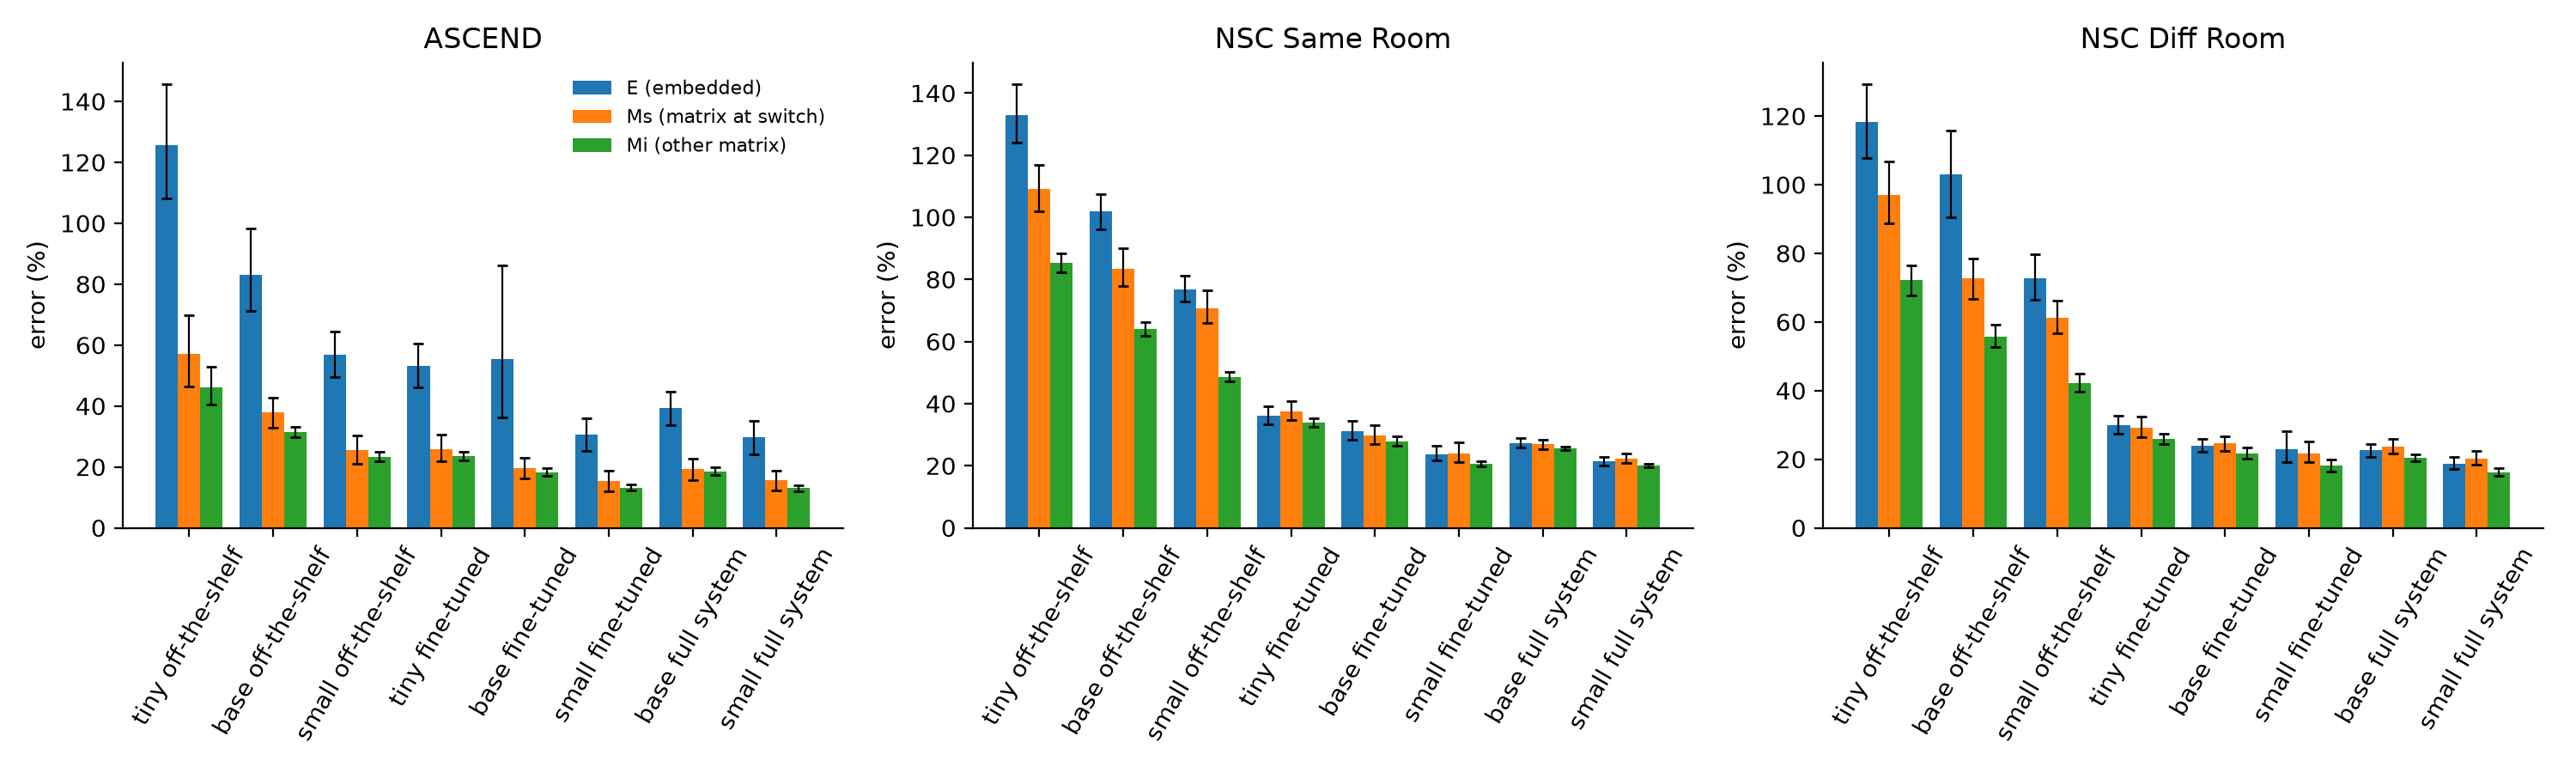
\includegraphics[width=0.9\textwidth]{fig2_role_errors.png}
  \caption{Error rate by role (\Emb, \Ms, \Mi) for each system on the three test sets. Embedded units have the highest error in almost every system.}
  \label{fig:roles}
\end{figure*}



\paragraph{Embedded units fail most.}
In almost every system and test set, embedded units have the highest error, followed by matrix units at a switch and then other matrix units (Figure~\ref{fig:roles}). For off-the-shelf small, embedded error is 56.8\% on ASCEND against 23.4\% for \Mi, and 76.7\% on NSC against 48.6\%.

\begin{table}[t]
\centering
\small
\setlength{\tabcolsep}{3pt}
\resizebox{\columnwidth}{!}{%
\begin{tabular}{lcccc}
\toprule
 & \multicolumn{2}{c}{Same word: \Emb{} $-$ matrix} & \multicolumn{2}{c}{Log-odds} \\
\cmidrule(lr){2-3}\cmidrule(lr){4-5}
System & English & Chinese & $b_{\text{emb}}$ & $b_{\text{emb}\times\text{en}}$ \\
\midrule
small, off-shelf & \textbf{+15.4} & \textbf{+26.0} & \textbf{0.94} & 0.09 \\
base, off-shelf & \textbf{+19.7} & \textbf{+32.0} & \textbf{1.18} & 0.23 \\
base, fine-tuned & \textbf{+8.0} & \textbf{+1.3} & 0.01 & \textbf{0.65} \\
small, fine-tuned & \textbf{+7.4} & +0.3 & $-$0.07 & \textbf{0.79} \\
\bottomrule
\end{tabular}}
\caption{Role vs.\ language. Left: error (points) on the same word type when embedded minus when in the matrix language. Right: logistic-regression coefficients (\S\ref{sec:rq1}). Bold: 95\% CI excludes 0.}
\label{tab:rq1}
\end{table}

\paragraph{The same word is harder when embedded.}
Table~\ref{tab:rq1} (left) compares each word type that occurs in both roles. For off-the-shelf small, an English word is 15.4 points [12.1, 18.6] more likely to be wrong when it is embedded than when it is part of an English-main sentence, and a Chinese character 26.0 points [23.9, 27.8] more. After fine-tuning, the gap for Chinese characters disappears (+0.3 for small) but the gap for English words remains (+7.4 [5.2, 10.1]).

To separate role from language, we fit a logistic regression on 46{,}916 units from 122 speakers:
\begin{equation}
\begin{split}
  \operatorname{logit} P(\text{err}) = {}& b_0 + b_{\text{emb}}\,\text{emb} + b_{\text{en}}\,\text{en} \\
  &+ b_{\text{emb}\times\text{en}}\,\text{emb}\cdot\text{en} \\
  &+ b_f \log f + b_d\, d + b_c\, \text{nsc},
\end{split}
\end{equation}
where emb, en and nsc are 1 if the unit is embedded, is English, or comes from NSC; $f$ is its training-data frequency and $d$ its spoken duration; CIs come from a speaker bootstrap.
Off the shelf, being embedded adds about one unit of log-odds over and above the unit's language ($b_{\text{emb}} = 0.94$ [0.78, 1.15] for small). After fine-tuning, $b_{\text{emb}}$ is about zero, so embedded Mandarin is no longer penalised, but the interaction for embedded English stays large ($0.79$ [0.42, 1.11] for small). \textbf{Fine-tuning removes the role penalty for embedded Mandarin but not for embedded English.}

\paragraph{Errors are transliterations, not translations.}
We expected many embedded errors to be translations. They are not: only 0.5--1.9\% of embedded units are replaced by a translation in the fine-tuned systems (3.4--4.0\% off the shelf). Far more often, the embedded English word is written as Chinese characters that sound like it (deadline$\rightarrow$\zh{得来}, python$\rightarrow$\zh{派森}). This affects up to 10.9\% of embedded units (off-the-shelf small on NSC 10.7\%; full small 2.5--3.8\%). The conclusion holds for every translation threshold $\tau \le 0.7$ (Appendix~\ref{sec:appendix}). A human audit of 30 random pairs confirms that translations are rare (none among the 26 labelled), but it labels most of the pairs our labels call transliterations as unrelated (\S\ref{sec:limitations}), so the transliteration rates are best read as upper bounds.

\section{RQ2: Methods at 16-bit}
\label{sec:rq2}

\begin{table*}[t]
\centering
\small
\begin{tabular}{lcccccc}
\toprule
 & \multicolumn{2}{c}{ASCEND} & \multicolumn{2}{c}{NSC Same Room} & \multicolumn{2}{c}{NSC Different Room} \\
\cmidrule(lr){2-3}\cmidrule(lr){4-5}\cmidrule(lr){6-7}
System & MER & \Emb & MER & \Emb & MER & \Emb \\
\midrule
small, off-the-shelf & 26.3 & 56.8 & 55.1 & 76.7 & 48.8 & 72.7 \\
tiny, FT & 26.1 & 53.2 & 34.5 & 36.2 & 26.8 & 29.8 \\
base, FT & 21.3 & 55.3 & 28.4 & 31.0 & 22.4 & 24.0 \\
small, FT & 14.8 & 30.6 & 21.4 & 23.8 & 19.0 & 22.9 \\
base, FT+L & 20.3 & 39.2 & 26.1 & 27.4 & 21.1 & 22.5 \\
small, FT+L & \textbf{14.6} & \textbf{29.8} & \textbf{20.6} & \textbf{21.3} & \textbf{17.1} & \textbf{18.7} \\
\bottomrule
\end{tabular}
\caption{Test error (\%) at 16-bit, greedy decoding. \Emb: embedded-word error. FT = ordinary fine-tuning; FT+L = fine-tuning with $\mathcal{L}_{\text{role}} + \lambda\mathcal{L}_{\text{sem}}$. Speaker-cluster 95\% CIs for small, FT+L: NSC Same Room MER [18.6, 23.4], Different Room [15.7, 18.6].}
\label{tab:main}
\end{table*}

\begin{table*}[t]
\centering
\small
\resizebox{\textwidth}{!}{%
\begin{tabular}{p{2mm}lcccccc}
\toprule
 & & \multicolumn{2}{c}{ASCEND} & \multicolumn{2}{c}{NSC Same Room} & \multicolumn{2}{c}{NSC Different Room} \\
\cmidrule(lr){3-4}\cmidrule(lr){5-6}\cmidrule(lr){7-8}
\multicolumn{2}{l}{System} & MER & \Emb & MER & \Emb & MER & \Emb \\
\midrule
\multicolumn{8}{l}{\emph{(a) Our losses vs.\ ordinary fine-tuning (FT) of the same size}} \\
 & base, role-weighted only & $-$0.7 & $-$14.6 & $-$0.6 & \textbf{$-$2.7} & $-$0.6 & \textbf{$-$0.9} \\
 & base, semantic only & $-$1.2 & $-$14.6 & \textbf{$-$1.3} & $-$1.7 & \textbf{$-$1.1} & $-$0.4 \\
 & base, FT+L (both) & $-$1.0 & $-$16.1 & \textbf{$-$2.3} & \textbf{$-$3.6} & \textbf{$-$1.3} & \textbf{$-$1.4} \\
 & small, role-weighted only & \textbf{$-$0.5} & $-$2.3 & +0.1 & $-$1.1 & $-$0.9 & $-$3.3 \\
 & small, FT+L (both) & $-$0.1 & $-$0.8 & \textbf{$-$0.7} & \textbf{$-$2.4} & \textbf{$-$1.9} & \textbf{$-$4.2} \\
\midrule
\multicolumn{8}{l}{\emph{(b) On-device gated re-ranking vs.\ the same model's greedy output}} \\
 & base, FT+L & \textbf{$-$0.7} & \textbf{$-$5.4} & \textbf{$-$0.4} & $-$0.4 & \textbf{$-$0.3} & $-$0.7 \\
 & small, FT+L & \textbf{$-$0.5} & \textbf{$-$3.9} & $-$0.1 & +0.2 & +0.1 & $-$0.1 \\
\bottomrule
\end{tabular}}
\caption{Paired differences in points (negative = better). The two panels use different baselines. Bold: 95\% CI of the difference excludes 0.}
\label{tab:deltas}
\end{table*}

\textbf{Answer: yes, but the gains are small; they are reliable on NSC and within noise on ASCEND (H2 partly supported).}

\paragraph{Fine-tuning matters most.}
Fine-tuning on ASCEND and NSC brings by far the largest gain, most of all on NSC, where off-the-shelf small has 55.1\% MER and small FT 21.4\% (Table~\ref{tab:main}).

\paragraph{Our losses help on NSC.}
Both losses lower embedded error, and together they work best (Table~\ref{tab:deltas}a). FT+L is significantly better than FT on both NSC test sets, for base and small, in both MER and embedded error, and its critical-word error does not rise. These gains (0.7--2.3 MER points) are larger than the 0.2 points by which a retrain of the same system moved. On ASCEND the changes are mostly within noise: there are only two test speakers, and a few long runs of repeated text dominate the embedded error. On our phone recordings, FT+L and FT are within noise of each other (small, embedded: $-$3.6 [$-$10.0, 2.7]). A direct penalty on transliterations did not help (Appendix~\ref{app:tl}).

\paragraph{Re-ranking helps only when gated.}
Re-ranking every clip lowers embedded error on Mandarin-main ASCEND (base FT+L, on-device: $-4.3$ points) but raises MER on English-main NSC (base FT+L, Different Room: $+0.5$; small FT+L, Same Room: $+0.8$). Gating fixes this (Table~\ref{tab:deltas}b). Only the 25--28\% of clips where the language-ID head hears a switch are re-ranked. The result is never significantly worse than greedy decoding, and for base FT+L it is significantly better on all three test sets in MER. Without the repetition filter, re-ranking fails badly, because candidates that repeat themselves win the length-normalised score. The head labels 95--98\% of speech frames correctly (Appendix~\ref{app:lid}).

\section{RQ3: Quantization}
\label{sec:rq3}

\textbf{Answer: 8-bit is safe; 4-bit hurts embedded words more in tiny and base; our repairs work in NF4 but not in whisper.cpp's 4-bit format (H3 supported for tiny and base).}

\begin{table}[t]
\centering
\small
\setlength{\tabcolsep}{2.6pt}
\resizebox{\columnwidth}{!}{%
\begin{tabular}{lllccc}
\toprule
Model & Format & Test set, main lang. & $\Delta_{\Emb}$ & $\Delta_M$ & $R$ \\
\midrule
tiny, FT & NF4 & ASCEND, Mandarin & +16.2 & +4.7 & 3.47 \\
base, FT & Q4\_0 & ASCEND, Mandarin & +8.2 & +1.9 & 4.40 \\
base, FT+L & Q4\_0 & ASCEND, Mandarin & +7.1 & +2.3 & 3.07 \\
base, FT+L & NF4 & NSC Same, English & +3.0 & +1.7 & 1.75 \\
tiny, FT & Q4\_0 & NSC Same, English & +8.9 & +6.4 & 1.40 \\
\bottomrule
\end{tabular}}
\caption{The five 4-bit settings whose 95\% CI of $R$ excludes 1, out of 20 reportable settings for tiny and base (FT and FT+L; NF4 and Q4\_0). $R>1$ in 14 of the 20 and the CI is below 1 in none. $\Delta$: change in error from the same backend's 16-bit run, in points; ``main lang.'' is the sentence's matrix language.}
\label{tab:R}
\end{table}

\paragraph{8-bit is safe.}
In every backend (LLM.int8, CTranslate2 int8, whisper.cpp Q8\_0) and model size, 8-bit causes no detectable extra harm to embedded words: no 8-bit $R$ has an interval above 1, and the matrix change is mostly within noise.

\paragraph{4-bit hurts embedded words more in tiny and base.}
For tiny and base, 4-bit raises embedded error 1.4 to 4.4 times as much as matrix error in the five settings where the interval of $R$ excludes 1 (Table~\ref{tab:R}; e.g.\ tiny FT in NF4 on ASCEND: $R=3.47$ [1.85, 6.13]). Across all 20 reportable tiny and base settings the direction is consistent: $R>1$ in 14 and significantly below 1 in none. This holds for embedded English (ASCEND) and embedded Mandarin (NSC), and in both NF4 and Q4\_0. Small is robust on the corpora: its errors change by about one point. In our per-block scan, the first encoder layer is always the most sensitive block.

\begin{table}[t]
\centering
\small
\setlength{\tabcolsep}{2.2pt}
\resizebox{\columnwidth}{!}{%
\begin{tabular}{lllcc}
\toprule
Repair & Model & Test set, main lang. & Loss & Rec [95\% CI] \\
\midrule
Mixed & base, FT & NSC Same, English & 2.5 & \textbf{0.86} [0.26, 2.99] \\
 & base, FT & NSC Diff, English & 3.5 & $-$0.00 [$-$1.10, 0.34] \\
 & tiny, FT & ASCEND, Mandarin & 16.2 & \textbf{0.65} [0.29, 0.91] \\
 & tiny, FT & NSC Same, English & 11.2 & \textbf{0.77} [0.40, 1.05] \\
 & tiny, FT & NSC Same, Mandarin & 17.3 & 0.33 [$-$1.12, 0.78] \\
 & tiny, FT & NSC Diff, English & 6.4 & \textbf{0.80} [0.28, 1.02] \\
 & base, FT+L & NSC Same, English & 3.0 & \textbf{0.70} [0.38, 1.04] \\
 & base, FT+L & NSC Same, Mandarin & 2.6 & 0.10 [$-$1.55, 0.98] \\
 & base, FT+L & NSC Diff, English & 2.2 & \textbf{0.48} [0.03, 0.90] \\
\midrule
QLoRA & base, FT & NSC Same, English & 2.5 & $-$0.30 [$-$3.64, 2.08] \\
 & base, FT & NSC Diff, English & 3.5 & 0.65 [$-$0.75, 1.05] \\
 & tiny, FT & ASCEND, Mandarin & 16.2 & \textbf{0.83} [0.57, 1.26] \\
 & tiny, FT & NSC Same, English & 11.2 & \textbf{0.72} [0.46, 0.98] \\
 & tiny, FT & NSC Same, Mandarin & 17.3 & \textbf{0.83} [0.39, 1.00] \\
 & tiny, FT & NSC Diff, English & 6.4 & 0.47 [$-$1.03, 0.92] \\
 & base, FT+L & NSC Same, English & 3.0 & \textbf{0.77} [0.54, 1.10] \\
 & base, FT+L & NSC Same, Mandarin & 2.6 & 0.22 [$-$0.75, 0.75] \\
 & base, FT+L & NSC Diff, English & 2.2 & 0.10 [$-$0.51, 0.47] \\
\bottomrule
\end{tabular}}
\caption{Recovery of the NF4 embedded-error loss, for every slice where the loss (points) has a CI excluding 0. Mixed precision keeps 1 (base FT), 2 (tiny FT) or 3 (base FT+L) blocks at 16-bit. Bold: CI of Rec excludes 0. After merging and re-quantizing to whisper.cpp Q4\_0, no slice has a Rec CI above 0.}
\label{tab:rec}
\end{table}

\paragraph{The repairs work in NF4 but not in the on-device format.}
Keeping the two or three most sensitive blocks at 16-bit, or adding QLoRA adapters, recovers about half to four-fifths of the NF4 embedded-error loss where it helps (Table~\ref{tab:rec}). For tiny FT and base FT+L, the recovery interval excludes 0 in 9 of the 14 affected slices. QLoRA does not help base FT, whose loss is small. When the adapters are merged into the weights and the model is re-quantized to whisper.cpp Q4\_0, the recovery disappears: no slice has a Rec interval above 0 (for tiny FT on NSC Same Room, English-main: $-$0.12; base FT+L: 0.06). The adapters were trained against NF4's grid, not Q4\_0's block-wise one, and whisper.cpp cannot load mixed-precision files at all. For whisper.cpp the answer is Q8\_0, which changes embedded error by at most 1.2 points for any fine-tuned model.


\begin{table}[t]
\centering
\small
\setlength{\tabcolsep}{3.5pt}
\begin{tabular}{lrrrrr}
\toprule
 & \multicolumn{2}{c}{16-bit} & \multicolumn{3}{c}{$\Delta_{\Emb}$} \\
\cmidrule(lr){2-3}\cmidrule(lr){4-6}
Model & MER & \Emb{} & Q8\_0 & NF4 & Q4\_0 \\
\midrule
small, off-the-shelf & 33.6 & 83.9 & & & \\
tiny, FT & 34.6 & 70.5 & +0.9 & +17.7 & +5.1 \\
base, FT & 23.0 & 49.7 & 0.0 & +5.5 & \textbf{+8.9} \\
base, FT+L & 24.4 & 50.7 & $-$0.4 & \textbf{+8.6} & \textbf{+7.2} \\
small, FT & 14.3 & 31.4 & $-$0.1 & +4.1 & $-$1.2 \\
small, FT+L & 13.4 & 27.8 & +1.3 & \textbf{+7.6} & +1.1 \\
\bottomrule
\end{tabular}
\caption{Our phone recordings (120 utterances, 3 readers). Error (\%) at 16-bit, and change in embedded error (points) to whisper.cpp Q8\_0, NF4 and whisper.cpp Q4\_0, each against its own backend's 16-bit run. Bold: 95\% CI excludes 0 (utterance bootstrap; optimistic with 3 readers).}
\label{tab:human}
\end{table}

\paragraph{On our phone recordings, 4-bit also hurts embedded words.}
8-bit again causes no detectable change: no 8-bit interval excludes 0 (Table~\ref{tab:human}), though with 227 embedded words the intervals reach up to about 4 points either side. At 4-bit, embedded error rises by 7--9 points for both base models (base FT, Q4\_0: +8.9 [2.9, 15.4]) and for small FT+L in NF4 (+7.6 [2.6, 13.3]), one of the four small-model 4-bit settings, while matrix error mostly does not change measurably (small FT+L: $-$1.4 [$-$3.1, 0.3]). So $R$ is mostly not reportable here. Tiny is dominated by repetition loops on single clips, so we draw no conclusion for it. These intervals are optimistic: there are three readers, and reader, phone and sentence are confounded.

\begin{table}[t]
\centering
\small
\setlength{\tabcolsep}{3.5pt}
\begin{tabular}{llrrrr}
\toprule
Model & Format & File & RSS & RTF & MER \\
\midrule
tiny, FT & Q8\_0 & 42 & 135 & 0.086 & 31.6 \\
base, FT+L & Q8\_0 & 78 & 196 & 0.176 & 25.8 \\
base, FT+L & Q4\_0 & 44 & 161 & 0.172 & 28.7 \\
base, FT+L & F16 & 141 & 261 & 0.336 & 25.7 \\
small, FT+L & Q8\_0 & 252 & 427 & 0.573 & 20.3 \\
small, FT+L & Q4\_0 & 139 & 315 & 0.584 & 21.0 \\
small, FT+L & CT2 int8 & 238 & 839 & 0.742 & 21.1 \\
small, FT+L & F16 & 465 & 650 & 1.299 & 20.3 \\
\bottomrule
\end{tabular}
\caption{Cost on a MacBook Pro (M2 Pro, 4 threads). File size and peak memory (RSS) in MB; RTF = processing time / audio time (below 1 is faster than real time); MER (\%) on the NSC Same Room CPU subset. Formats are whisper.cpp unless marked CT2 (CTranslate2).}
\label{tab:speed}
\end{table}

\paragraph{Cost on a laptop.}
whisper.cpp Q8\_0 is as fast as Q4\_0, as accurate as F16 and about half its size (Table~\ref{tab:speed}): small FT+L is a 252\,MB file with RTF 0.57 and 20.3\% MER. The language-ID head raises base's RTF from 0.21 to 0.30 (CTranslate2). Re-ranking every clip raises it to 1.76; with gating, which re-ranks about a quarter of clips, we estimate about 0.7 but did not measure it.

\section{Example Outputs}
\label{sec:examples}

Table~\ref{tab:examples} shows 16 of our phone recordings drawn at random. Off-the-shelf small keeps most embedded English in Mandarin-main sentences (insulin, module, release) but loses embedded Mandarin in English-main ones, writing it as English sound-alikes (\zh{身份证}$\rightarrow$``shuffling jump'', \zh{贷款}$\rightarrow$``Taekwun''). Small FT+L fixes most of these but still fails on rare terms (\zh{布洛芬}$\rightarrow$\zh{不落分}, \zh{会议室}$\rightarrow$``hui yi shah'', prednisolone, polyclinic$\rightarrow$polytechnic), and once repeats a phrase instead of the sentence. In NF4 most outputs are unchanged; it adds errors on \zh{身份证} (written \zh{身分证}) and \zh{期末考}, and happens to avoid the repeated phrase.

\begin{table*}[t]
\centering
\footnotesize
\setlength{\tabcolsep}{3pt}
\begin{tabular}{*{4}{>{\raggedright\arraybackslash}p{0.235\textwidth}}}
\toprule
Reference (what was said) & Small, off-the-shelf, 16-bit & Small FT+L, 16-bit & Small FT+L, NF4 \\
\midrule
\zh{我\hspace{0pt}们\hspace{0pt}约\hspace{0pt}了} polyclinic \zh{下\hspace{0pt}午\hspace{0pt}三\hspace{0pt}点\hspace{0pt}半} & \zh{我\hspace{0pt}們\hspace{0pt}約\hspace{0pt}了}POLI\-TIC\-NIC\zh{下\hspace{0pt}午}3\zh{點\hspace{0pt}半} \textsuperscript{1} & \zh{我\hspace{0pt}们\hspace{0pt}约\hspace{0pt}了} polytechnic \zh{下\hspace{0pt}午} 3 \zh{点\hspace{0pt}半} \textsuperscript{1} & \zh{我\hspace{0pt}们\hspace{0pt}圆\hspace{0pt}了} polytechnic \zh{下\hspace{0pt}午} 3 \zh{点\hspace{0pt}半} \textsuperscript{1} \\
\zh{护\hspace{0pt}士\hspace{0pt}说} vaccine \zh{打\hspace{0pt}完\hspace{0pt}要\hspace{0pt}等\hspace{0pt}十\hspace{0pt}五\hspace{0pt}分\hspace{0pt}钟} & \zh{護\hspace{0pt}士\hspace{0pt}說}, vaccine \zh{打\hspace{0pt}完\hspace{0pt}要\hspace{0pt}等} 15 \zh{分\hspace{0pt}鐘} \textsuperscript{0} & \zh{抢\hspace{0pt}了} 15 \zh{分\hspace{0pt}钟\hspace{0pt}抢\hspace{0pt}了} 15 \zh{分\hspace{0pt}钟} \textsuperscript{1} & \zh{忽\hspace{0pt}视\hspace{0pt}说} vaccine \zh{打\hspace{0pt}完\hspace{0pt}要\hspace{0pt}等} 15 \zh{分\hspace{0pt}钟} \textsuperscript{0} \\
\zh{这\hspace{0pt}个} python script \zh{跑\hspace{0pt}了\hspace{0pt}四\hspace{0pt}十\hspace{0pt}分\hspace{0pt}钟} & \zh{这\hspace{0pt}个\hspace{0pt}排\hspace{0pt}队}script\zh{跑\hspace{0pt}了}40\zh{分\hspace{0pt}钟} \textsuperscript{2} & \zh{这\hspace{0pt}个} python script \zh{跑\hspace{0pt}了} 40 \zh{分\hspace{0pt}钟} \textsuperscript{0} & \zh{这\hspace{0pt}个} python script \zh{跑\hspace{0pt}了} 40 \zh{分\hspace{0pt}钟} \textsuperscript{0} \\
\zh{你\hspace{0pt}记\hspace{0pt}得\hspace{0pt}带} insulin \zh{去\hspace{0pt}，\hspace{0pt}放\hspace{0pt}在\hspace{0pt}冰\hspace{0pt}箱\hspace{0pt}第\hspace{0pt}二\hspace{0pt}层} & \zh{你\hspace{0pt}記\hspace{0pt}得\hspace{0pt}帶} Insulin \zh{區\hspace{0pt}放\hspace{0pt}在\hspace{0pt}冰\hspace{0pt}箱\hspace{0pt}第\hspace{0pt}二\hspace{0pt}重} \textsuperscript{0} & \zh{你\hspace{0pt}记\hspace{0pt}得\hspace{0pt}带} insulin \zh{去\hspace{0pt}放\hspace{0pt}在\hspace{0pt}冰\hspace{0pt}箱\hspace{0pt}第\hspace{0pt}二\hspace{0pt}从} \textsuperscript{0} & \zh{你\hspace{0pt}记\hspace{0pt}得\hspace{0pt}带} insulin \zh{去\hspace{0pt}放\hspace{0pt}在\hspace{0pt}冰\hspace{0pt}箱\hspace{0pt}第\hspace{0pt}二\hspace{0pt}从} \textsuperscript{0} \\
\zh{这\hspace{0pt}个} module \zh{的} quiz \zh{占\hspace{0pt}百\hspace{0pt}分\hspace{0pt}之\hspace{0pt}二\hspace{0pt}十} & \zh{這\hspace{0pt}個}Module\zh{的}Quiz,\zh{占}20\% \textsuperscript{0} & \zh{这\hspace{0pt}个} module \zh{的} quiz \zh{占\hspace{0pt}百\hspace{0pt}分\hspace{0pt}之\hspace{0pt}二\hspace{0pt}十} \textsuperscript{0} & \zh{这\hspace{0pt}个} module \zh{的} quiz \zh{占\hspace{0pt}百\hspace{0pt}分\hspace{0pt}之\hspace{0pt}二\hspace{0pt}十} \textsuperscript{0} \\
\zh{这\hspace{0pt}个} bug \zh{要\hspace{0pt}在} release \zh{之\hspace{0pt}前} fix & \zh{这\hspace{0pt}个}bug\zh{要\hspace{0pt}在}release\zh{之\hspace{0pt}前}fix\zh{。} \textsuperscript{0} & \zh{这\hspace{0pt}个} bug \zh{要\hspace{0pt}在} release \zh{之\hspace{0pt}前} fix \textsuperscript{0} & \zh{这\hspace{0pt}个} bug \zh{要\hspace{0pt}在} release \zh{之\hspace{0pt}前} fix \textsuperscript{0} \\
\zh{医\hspace{0pt}生\hspace{0pt}说} prednisolone \zh{要\hspace{0pt}慢\hspace{0pt}慢\hspace{0pt}减\hspace{0pt}量} & \zh{醫\hspace{0pt}生\hspace{0pt}說},Pretinicillin\zh{要\hspace{0pt}慢\hspace{0pt}慢\hspace{0pt}解\hspace{0pt}釋} \textsuperscript{1} & \zh{医\hspace{0pt}生\hspace{0pt}说} pratnicillin your \zh{慢\hspace{0pt}慢\hspace{0pt}减\hspace{0pt}凉} \textsuperscript{1} & \zh{医\hspace{0pt}生\hspace{0pt}说} pratnicillin your \zh{慢\hspace{0pt}慢\hspace{0pt}减\hspace{0pt}量} \textsuperscript{1} \\
\zh{那\hspace{0pt}个} report \zh{要\hspace{0pt}写\hspace{0pt}三\hspace{0pt}千\hspace{0pt}个\hspace{0pt}字} & \zh{那\hspace{0pt}个}report\zh{要\hspace{0pt}写}3000\zh{个\hspace{0pt}字} \textsuperscript{0} & \zh{那\hspace{0pt}个} report \zh{要\hspace{0pt}写} 3000 \zh{个\hspace{0pt}字} \textsuperscript{0} & \zh{那\hspace{0pt}个} report \zh{要\hspace{0pt}写} 3000 \zh{个\hspace{0pt}字} \textsuperscript{0} \\
\midrule
the \zh{药\hspace{0pt}房} closes at nine tonight & The yellow phone closes at 9pm tonight. \textsuperscript{2} & the \zh{药\hspace{0pt}房} closes at nine tonight \textsuperscript{0} & the \zh{药\hspace{0pt}房} closes at nine tonight \textsuperscript{0} \\
the nurse said \zh{布\hspace{0pt}洛\hspace{0pt}芬} only after meals & The nurse said bull often only after meals. \textsuperscript{3} & the nurse said \zh{不\hspace{0pt}落\hspace{0pt}分} only after meals \textsuperscript{3} & dinner set \zh{不\hspace{0pt}落\hspace{0pt}分} only after meals \textsuperscript{3} \\
he forgot the \zh{门\hspace{0pt}卡} so he could not enter level five & He forgot the Munkah so he could not answer level 5. \textsuperscript{2} & he forgot the \zh{门\hspace{0pt}卡} so he could not answer level five \textsuperscript{0} & he forgot the \zh{门\hspace{0pt}卡} so he could not answer level five \textsuperscript{0} \\
please bring your \zh{身\hspace{0pt}份\hspace{0pt}证} for the exam & Please remember to bring your shuffling jump for the exam. \textsuperscript{3} & please remember to bring your \zh{身\hspace{0pt}份\hspace{0pt}证} for the exam \textsuperscript{0} & please remember to bring your \zh{身\hspace{0pt}分\hspace{0pt}证} for the exam \textsuperscript{1} \\
my mother keeps the \zh{药} in the second drawer & My mother keeps the yao in the second drawer. \textsuperscript{1} & my mother keeps the \zh{药} in the second drawer \textsuperscript{0} & my mother keeps the \zh{药} in the second drawer \textsuperscript{0} \\
I booked the \zh{会\hspace{0pt}议\hspace{0pt}室} from two to four & I bought the Huyish from 2 to 4. \textsuperscript{3} & i book the hui yi shah from two to four \textsuperscript{3} & i book the hui yi shah from two to four \textsuperscript{3} \\
the \zh{贷\hspace{0pt}款} has twelve monthly payments & The Taekwun has 12 monthly payments. \textsuperscript{2} & the \zh{贷\hspace{0pt}款} has twelve monthly payments \textsuperscript{0} & the \zh{贷\hspace{0pt}款} has twelve monthly payments \textsuperscript{0} \\
the \zh{期\hspace{0pt}末\hspace{0pt}考} starts on the first of December & The team who caused that on the 1st of December \textsuperscript{3} & the \zh{齐\hspace{0pt}木\hspace{0pt}考} starts on the first of december \textsuperscript{2} & the \zh{起\hspace{0pt}目\hspace{0pt}靠} start on the first of december \textsuperscript{3} \\
\bottomrule
\end{tabular}
\caption{Sixteen of our phone recordings drawn at random (seed 425; top: Mandarin-main, bottom: English-main) and the raw outputs of three systems. Superscript: number of embedded words the system got wrong in that clip. Off-the-shelf Whisper often writes Traditional characters, which the normaliser maps to Simplified before scoring.}
\label{tab:examples}
\end{table*}


\section{Applications}
\label{sec:apps}

We wrote our phone recordings around names, numbers, drug and course terms, and the clips in Table~\ref{tab:examples} point to settings where an on-device, code-switching recogniser is useful and where the embedded word carries the content:
\begin{itemize}
  \item \textbf{Clinics and pharmacies.} Notes or patient instructions such as ``\zh{医生说} prednisolone \zh{要慢慢减量}'' or ``the nurse said \zh{布洛芬} only after meals''. Patient audio should stay on the device, and the drug name is exactly the word a wrong transcript must not lose.
  \item \textbf{Live captions for deaf and hard-of-hearing users} in lectures, tutorials and meetings, where course codes and technical terms (module, quiz, release) are embedded in Mandarin speech. Captions must keep up with speech: small FT+L in 8-bit runs at RTF 0.57 on a laptop CPU.
  \item \textbf{Banking, government and telco hotlines}, where callers mix in words like \zh{身份证} or \zh{贷款} over a phone line. Our phone recordings show that off-the-shelf Whisper writes these as English sound-alikes, while the fine-tuned models get them right.
  \item \textbf{Eldercare and family use}, e.g.\ voice reminders like ``my mother keeps the \zh{药} in the second drawer''. A home device should not stream household speech to the cloud, and it must still work without a fast network connection.
  \item \textbf{Personal dictation} of messages, notes and reminders (``the \zh{期末考} starts on the first of December''), where a missed embedded word loses the one fact the note was written to keep.
\end{itemize}

\paragraph{Conversational use.} The same recogniser can be the input to a spoken assistant: the user speaks, the on-device model transcribes each turn, a language model reads the transcript and writes a reply, and a speech synthesiser reads that reply aloud. In such a dialogue the embedded word is often the slot the assistant must act on (the drug, the date, the room), so the role-based error we measure matters more than overall MER. A dropped embedded word does not produce an obviously broken transcript. It produces a fluent sentence that the language model will answer confidently and wrongly (``bring your shuffling jump'' instead of \zh{身份证}). Our language-ID head can also help here: it tells the assistant which language each part of the turn was in, so the reply can follow the user's mix, and, because our best system still misses about one embedded word in five on NSC, the assistant can read back an embedded word before acting on it (``Prednisolone, is that right?'').

Turn-taking sets the speed budget. At RTF 0.57, a 5-second turn takes about 3\,s to transcribe on our laptop, which is too slow for a natural reply; base at RTF 0.21 (CTranslate2) takes about 1\,s, and gated re-ranking adds cost only on the quarter of turns with a switch. A conversational system would therefore pair a smaller or streaming recogniser with our loss and gating methods, and could pass the previous turns to Whisper as a text prompt so that terms already mentioned in the dialogue are more likely to be recognised again. We have not tested these designs; they are directions this work makes possible, not results.

\section{Conclusion}
\label{sec:conclusion}

One overall error rate hides how speech recognisers treat the words that carry the meaning in code-switched speech. Splitting errors by role answers our three questions:
\begin{itemize}
  \item \textbf{H1, supported.} Embedded words fail more often than the same words in the matrix language. Fine-tuning closes this gap for embedded Mandarin but not for embedded English. Errors are rarely translations.
  \item \textbf{H2, partly supported.} Our two losses and gated language-ID re-ranking give small but reliable gains on NSC; on ASCEND and our recordings they are within noise.
  \item \textbf{H3, supported for tiny and base.} 4-bit hurts embedded words more than other words; our repairs work in NF4 but not in whisper.cpp's 4-bit format.
\end{itemize}
\textbf{Recommendation:} on device, use 8-bit. It caused no detectable harm in any backend, and in whisper.cpp it is as fast as 4-bit.

Future work: more speakers and unprompted switching; losses that act on every embedded word rather than on whole candidates; and repairs trained on the deployed format's own grid.


\section*{Individual Contributions}
All four members contributed to the project.

\noindent\textbf{Rui Cong}: text normaliser, unit splitter and role labels; the role scorer, metrics, bootstrap intervals, $R$ and Rec; data loaders (with Nibras); read 40 of our phone sentences; translation-label audit; checked \S\ref{sec:task}.

\noindent\textbf{Phoebe}: training code: fine-tuning, the role-weighted and semantic losses; read 40 phone sentences; critical-word audit; checked \S\ref{sec:methods} and \S\ref{sec:rq2}.

\noindent\textbf{Bridgette}: forced alignment, language-ID head, N-best re-ranking and gating; alignment checks and speed harness; read 40 phone sentences; checked \S\ref{sec:setup}.

\noindent\textbf{Nibras}: team lead; NSC Part~4 access and preparation; quantization (bitsandbytes, CTranslate2 and whisper.cpp exports, sensitivity scan, QLoRA); ran the phone-recording tests; drafted this report.

\section*{Limitations}
\label{sec:limitations}

\paragraph{Prompted switching.} NSC speakers were asked to switch languages, and they switch more often within an utterance and in longer spans than ASCEND speakers (\S\ref{sec:data}), so their switching may be more deliberate than natural code-switching.

\paragraph{Small ASCEND test set.} ASCEND test has two speakers, so its utterance-level intervals are optimistic and several ASCEND differences are within noise. NSC claims use speaker-cluster intervals.

\paragraph{Automatic labels.} The translation, transliteration and critical-word labels, and the check for partner speech leaking into NSC recordings, come from two LLM annotators with adjudication or from signal rules, not from people. The transliteration threshold ($\theta=0.1$) is loose: for long words, one shared consonant code can be enough. Agreement is reported in Appendix~\ref{app:labels} (translation vs.\ rest $\kappa=0.84$; critical words $\kappa=0.77$; leakage rule vs.\ annotator $\kappa=0.29$). Two team members each audited a small sample, which we take as the final human check. On 26 random translation pairs, the human agreed with our labels on 58\% [39, 77] ($\kappa=0.15$ [0.00, 0.40]): neither side found a translation, but the human called 11 of the 13 pairs our labels call transliterations unrelated, so our transliteration rates are likely too high. On 50 critical-word candidates drawn from cases where the rule tagger and the LLM annotators disagreed, agreement with the adjudicated list was 66\% [54, 78] ($\kappa=0.32$ [0.12, 0.55]); the human was stricter, rejecting 15 of the 38 words the list marks critical. Both audits have one annotator and few items (95\% bootstrap intervals over items), and the partner-leakage labels were not audited.

\paragraph{Small set of phone recordings.} Our phone recordings (\S\ref{sec:data}) are 120 read sentences from three readers, each reading different sentences once, so reader, phone and sentence are confounded, intervals are utterance bootstraps and optimistic, and most fragility ratios are not reportable. In 24 clips all fine-tuned models make the same error; besides shared misrecognitions (\emph{opens}$\rightarrow$\emph{open}), these include homophones no recogniser can resolve (\zh{她}/\zh{他}) and normaliser mismatches (\emph{level 3} vs.\ \emph{three}) that slightly inflate every system's error. The earlier synthetic stress set (CosyVoice~2) is kept in the appendix for comparison only.

\paragraph{One training run per system.} Each system was trained once. A retrain of the same base system moved test MER by at most 0.2 points, smaller than the gains we report, but we did not retrain small.

\paragraph{Scope of speed results.} Speed was measured on one machine (Apple M2 Pro); the relative order of formats may differ on x86 or phone processors. Gated re-ranking speed is an estimate from its parts.

\section*{Ethics and Data Licences}

We use NSC Part~4 under the Singapore Open Data Licence version 1.0, which asks for the following notice: \emph{Contains information from the National Speech Corpus (Part~4) accessed on 14 October 2026 from the Infocomm Media Development Authority of Singapore (IMDA), which is made available under the terms of the Singapore Open Data Licence version 1.0 (\url{https://data.gov.sg/open-data-licence}).} We use the data for research only and do not suggest that IMDA endorses this work. ASCEND and FLEURS are used under their published licences, and the synthetic stress-set voices were produced with CosyVoice~2 (Apache-2.0) from FLEURS prompts (CC-BY 4.0). The human stress recordings were made by three of the authors, who agreed to their use for this project; they are shared only with the course staff as part of the submission and are not released publicly. We collected no data from people outside the team. Speech recognition that runs on the device keeps audio off remote servers, which matters for the clinical and counselling uses that motivate this work; errors on names, numbers and drug terms in such settings can still cause harm, so outputs should be checked by a person where mistakes matter.


\bibliography{refs}

\appendix
\section{Additional Results}
\label{sec:appendix}

\subsection{Hyperparameter selection}\label{app:grid}
Grids were run on base and scored on pooled ASCEND + NSC validation (Table~\ref{tab:grid}). Role weights: lowest embedded error among runs whose MER is at most 1 point above plain fine-tuning. Semantic loss: lowest semantic MER among runs whose critical-word error does not rise.

\begin{table}[h]
\centering
\small
\setlength{\tabcolsep}{3pt}
\begin{tabular}{lcccc}
\toprule
Run & MER & \Emb & CWER & Chosen \\
\midrule
plain fine-tuning & 31.42 & 36.13 & 27.91 & \\
$\alpha{=}0.5, \beta{=}0$ & 31.57 & 35.04 & 28.35 & \\
$\alpha{=}0.5, \beta{=}0.5$ & 30.44 & 33.50 & 27.91 & \checkmark \\
$\alpha{=}1, \beta{=}0$ & 34.34 & 44.82 & 27.47 & \\
$\alpha{=}1, \beta{=}0.5$ & 31.28 & 33.90 & 29.45 & \\
$\alpha{=}2, \beta{=}0$ & 32.49 & 33.69 & 28.57 & \\
$\alpha{=}2, \beta{=}0.5$ & 32.81 & 37.02 & 29.01 & \\
\midrule
$\lambda{=}0.1, \rho_0{=}0.2$ & 29.41 & 33.02 & 25.49 & \\
$\lambda{=}0.1, \rho_0{=}0.5$ & 29.39 & 33.22 & 26.81 & \checkmark \\
$\lambda{=}0.3, \rho_0{=}0.2$ & 29.62 & 33.33 & 27.03 & \\
$\lambda{=}0.3, \rho_0{=}0.5$ & 29.44 & 33.06 & 26.59 & \\
\bottomrule
\end{tabular}
\caption{Validation grids on base (\%). Semantic-loss runs use $\alpha=\beta=0.5$.}
\label{tab:grid}
\end{table}

\subsection{Language-ID head}\label{app:lid}
\begin{table}[h]
\centering
\small
\setlength{\tabcolsep}{3pt}
\resizebox{\columnwidth}{!}{%
\begin{tabular}{lccc}
\toprule
Head & Accuracy (\%) & Boundary (ms) & Found (\%) \\
\midrule
shared (base FT) & 96.0 / 95.4 & 60 / 120 & 75 / 85 \\
own, base FT+L & 95.9 / 95.3 & 60 / 100 & 77 / 84 \\
own, small FT+L & 97.7 / 96.4 & 20 / 80 & 78 / 85 \\
\bottomrule
\end{tabular}}
\caption{Language-ID head on validation (ASCEND / NSC). Accuracy on speech frames; median distance from a true switch to the nearest predicted one; share of switches detected.}
\label{tab:lid}
\end{table}
The model's own head gives the same re-ranking accuracy as the shared head; its benefit is speed, because it reuses the model's encoder pass.

\subsection{Label agreement and the translation threshold}\label{app:labels}
Two LLM annotators labelled each item independently, the second seeing only the written rubric. On 1{,}768 ASCEND pairs, agreement was 0.798 ($\kappa=0.62$) over three classes and 0.981 ($\kappa=0.84$) for translation vs.\ the rest. On 335 candidate critical-word types, agreement was 0.899 ($\kappa=0.77$); the rule tagger agreed less with either annotator ($\kappa=0.55$ and $0.47$), mostly because it has no named-entity component. Human audits of small samples agree less with these labels ($\kappa=0.15$ for translation labels, $n=26$; $\kappa=0.32$ for critical words, $n=50$; see Limitations); results table 20c lists every comparison with its interval. With $\tau$ between 0.6 and 0.7 the number of flagged translation occurrences changes by about $\pm$20\%, and translations remain a small share of embedded errors for every $\tau \le 0.7$.

\subsection{Partner speech and alignment}\label{app:partner}
In NSC Same Room recordings the partner's voice is sometimes audible. A signal rule (overlap with the partner's transcript, speaker-embedding similarity, and output words that appear in the partner's transcript) flags 1.75\% of Same Room and 0.15\% of Different Room test utterances. Removing them lowers Same Room MER by about one point for every fine-tuned model (small FT+L: 20.65 $\rightarrow$ 19.71) and changes no conclusion. Forced-alignment boundaries are within a median of 10\,ms of known switches in FLEURS splices (87\% within 50\,ms) and a median of 73\,ms from Whisper's cross-attention times at real switches.

\subsection{Training on Different Room audio}\label{app:diffroom}
\begin{table}[h]
\centering
\small
\setlength{\tabcolsep}{3pt}
\begin{tabular}{lcc}
\toprule
NSC training data (40\,h) & Same test & Diff (held-out) \\
\midrule
Same Room (= base FT) & 28.4 & 21.6 \\
Different Room & 32.3 & 23.6 \\
20\,h Same + 20\,h Diff & 28.3 & 22.2 \\
\bottomrule
\end{tabular}
\caption{MER (\%) of base when NSC training audio comes from the Different Room condition (Different Room split by session; ASCEND training data unchanged).}
\label{tab:diffroom}
\end{table}
Training on Different Room audio does not help on Different Room test speech: training only on it is 2.0 points worse [0.4, 3.8] (Table~\ref{tab:diffroom}). The gap between the two rooms in Table~\ref{tab:main} is therefore not a mismatch between training and test conditions.

\subsection{Transliteration penalty}\label{app:tl}
To target transliterations directly, we added an extra cost to each candidate of the semantic loss:
\begin{equation}
  c_{\text{tl}}(y) = c(y) + \gamma\, N_{\text{tl}}(y),
\end{equation}
where $c(y)$ is the semantic cost (\S\ref{sec:methods}), $N_{\text{tl}}(y)$ is the number of embedded reference words that $y$ writes as a sound-alike in the other script (\S\ref{sec:data}), and $\gamma$ is the extra weight; $\gamma=0$ gives the semantic loss back. We tested it on base in two rounds: $\gamma \in \{0.5, 1\}$ at $\lambda=0.1$, then $\lambda \in \{0.4, 1\} \times \gamma \in \{0, 3\}$. Each round included a $\gamma=0$ retrain to measure run-to-run noise (the ``control'' rows of Table~\ref{tab:tl}). The penalty did not lower transliteration, MER or embedded error on any test set. Its gradient was about 1/130 of the role-weighted loss's, because it acts only when a sampled candidate contains a transliteration; raised to match the main loss ($\lambda=1$, $\gamma=3$), it still did not beat FT+L.
\begin{table}[h]
\centering
\small
\setlength{\tabcolsep}{2.5pt}
\resizebox{\columnwidth}{!}{%
\begin{tabular}{lcccccc}
\toprule
 & \multicolumn{3}{c}{MER} & \multicolumn{3}{c}{Transliteration rate} \\
\cmidrule(lr){2-4}\cmidrule(lr){5-7}
Run & A & S & D & A & S & D \\
\midrule
$\lambda{=}0.1$, $\gamma{=}0$ (control) & $-$0.14 & $-$0.09 & $-$0.08 & +0.91 & $-$0.07 & +0.21 \\
$\lambda{=}0.1$, $\gamma{=}0.5$ & $-$0.27 & +0.17 & \textbf{+0.31} & +0.13 & +0.05 & $-$0.39 \\
$\lambda{=}0.1$, $\gamma{=}1$ & $-$0.37 & $-$0.04 & $-$0.02 & $-$0.65 & $-$0.25 & $-$0.05 \\
$\lambda{=}1$, $\gamma{=}0$ (control) & $-$0.12 & $-$0.06 & +0.16 & +0.39 & $-$0.31 & $-$0.05 \\
$\lambda{=}1$, $\gamma{=}3$ (chosen) & +0.12 & +0.26 & +0.19 & +0.26 & $-$0.04 & $-$0.27 \\
\bottomrule
\end{tabular}}
\caption{Transliteration penalty on base: paired test differences vs.\ base FT+L (points; negative = better). A = ASCEND, S = NSC Same Room, D = NSC Different Room. Bold: CI excludes 0. Embedded error changes are not significant for any penalised run.}
\label{tab:tl}
\end{table}
At $\lambda=0.1$, no $\gamma$ passed the validation rule (MER at most 0.5 points and critical-word error no higher than FT+L), so small was not trained. In the second round the rule allowed critical-word error up to 1 point higher, the size of the first round's retrain noise; only $\lambda=1, \gamma=3$ qualified, although it had the highest validation transliteration rate.

\begin{table*}[t]
\centering
\scriptsize
\begin{verbatim}
# 0. Environment: Python 3.11, one CUDA GPU (CPU formats need ctranslate2 and whisper.cpp)
micromamba create -n cs425 -c conda-forge python=3.11 pip ffmpeg && micromamba activate cs425
pip install -r requirements.txt && pip install -e . && pytest        # normaliser + scorer tests
# 1. Pre-processing: 16 kHz mono FLAC clips + JSONL manifests in data/<corpus>/manifests/
huggingface-cli download CAiRE/ASCEND --repo-type dataset --local-dir data/ascend/hf
python scripts/prepare_ascend.py                       # official splits
python scripts/fetch_nsc_dropbox.py fetch data/nsc_part4 -j 2 --only cs-chn && python scripts/prepare_nsc.py
python scripts/prepare_fleurs.py                       # spliced clips for the language-ID head
python scripts/prepare_stress.py                       # our recordings: data/stress/audio/<reader>/<id>.wav
python scripts/align.py ascend_train nsc_train ascend_val nsc_val    # MMS word times
# 2. Training (checkpoints in ckpt/<run>/best)
python scripts/train.py configs/ft_base.yaml           # FT; also ft_tiny.yaml, ft_small.yaml
python scripts/train.py configs/ft_base.yaml --run full_base --alpha 0.5 --beta 0.5 --lambda_sem 0.1 --rho0 0.5
python scripts/train_lid.py --encoder ckpt/ft_base/best --run lid_ft_base
python scripts/train.py configs/ft_base.yaml --run qat_full_base --model ckpt/full_base/best \
       --lora true --lr 1e-4 --epochs 1 --warmup 100
# 3. Testing (predictions in preds/<model>__<precision>__<method>.jsonl)
python scripts/decode.py --model ckpt/full_base/best --model_tag full_base --precision nf4_bnb --method full
python scripts/deploy_eval.py --model ckpt/full_base/best --tag full_base --method full \
       --formats ct2_f32 ct2_int8 ggml_f16 ggml_q8_0 ggml_q4_0
python scripts/sensitivity.py --model ckpt/full_base/best --tag full_base      # mixed-precision blocks
python scripts/rerank.py --model ckpt/full_base/best --tag full_base --lid ckpt/lid_ft_base/head.pt --loop_filter
# 4. Scoring and tables (results/tables/*.csv, results/figures/)
python scripts/score.py full_base__fp16__full full_base__nf4_bnb__full     # all metrics, 95% CIs
python scripts/score.py --fragility full_base__fp16__full full_base__nf4_bnb__full --set nsc_test --main en
python scripts/make_results.py && python scripts/export_tables.py && python scripts/make_figures.py
GPU=0 bash scripts/pipeline.sh stress_human && python scripts/make_human_tables.py   # phone recordings
\end{verbatim}
\vspace{-1em}
\caption{Commands to pre-process the data, train, test and score (run from the repository root; GPU chosen with \texttt{CUDA\_VISIBLE\_DEVICES}). \texttt{scripts/pipeline.sh <stage>} chains these steps with the settings we used; \texttt{DRY=1} prints the commands.}
\label{tab:commands}
\end{table*}

\subsection{Synthetic stress set}\label{app:synth}
We synthesised 120 code-switched sentences rich in critical words with CosyVoice~2 in four voices, clean and through a simulated phone channel (300--3400\,Hz, 8\,kHz, room reverberation, 20\,dB noise). The phone channel roughly doubles errors and embedded words suffer most (small FT+L: MER 22.3\% clean, 36.8\% phone; embedded error 54.6\% and 74.5\%). Embedded error is high even on clean speech: the same sentences read by people give 15--27 points lower embedded error for every fine-tuned model (\S\ref{sec:rq3}), which confirms that the synthetic voices often mispronounce embedded words. This set therefore supports only relative comparisons.



\subsection{Logistic regression for RQ1}\label{app:reg}
To separate role from language, we fit
\begin{equation}
\begin{split}
  \operatorname{logit} P(\text{err}) = {}& b_0 + b_{\text{emb}}\,\text{emb} + b_{\text{en}}\,\text{en} \\
  &+ b_{\text{emb}\times\text{en}}\,\text{emb}\cdot\text{en} \\
  &+ b_f \log f + b_d\, d + b_c\, \text{nsc},
\end{split}
\end{equation}
where emb, en and nsc are 1 if the unit is embedded, is English, or comes from NSC (else 0); $f$ is the unit's frequency in the training data and $d$ its spoken duration; and each $b$ is a coefficient. It is fit on 46{,}916 units from 122 speakers, with CIs from a speaker bootstrap (Table~\ref{tab:reg}). $b_{\text{emb}}$ is the effect of being embedded for a Chinese character; for an English word it is $b_{\text{emb}} + b_{\text{emb}\times\text{en}}$.

\begin{table}[h]
\centering
\small
\begin{tabular}{lcc}
\toprule
System & $b_{\text{emb}}$ & $b_{\text{emb}\times\text{en}}$ \\
\midrule
small, off-the-shelf & \textbf{0.94} & 0.09 \\
base, off-the-shelf & \textbf{1.18} & 0.23 \\
base, FT & 0.01 & \textbf{0.65} \\
small, FT & $-$0.07 & \textbf{0.79} \\
\bottomrule
\end{tabular}
\caption{Logistic-regression coefficients (log-odds). Bold: 95\% CI excludes 0.}
\label{tab:reg}
\end{table}

\subsection{How to run}\label{app:run}
Table~\ref{tab:commands} lists the commands, run from the root of \url{https://github.com/nibess1/cs425_codeswitch}. \emph{Pre-processing} turns each corpus into 16\,kHz FLAC clips and a JSONL manifest (raw and normalised reference, speaker, main language, duration). \emph{Training} reads a YAML config whose fields can be overridden on the command line (Table~\ref{tab:hparams}). \emph{Testing} decodes the test sets with a 16-bit, simulated 8/4-bit (bitsandbytes) or exported CPU model (CTranslate2, whisper.cpp) and writes one JSONL line per utterance. \emph{Scoring} (\texttt{score.py}) computes every metric of \S\ref{sec:task} with bootstrap intervals.




\end{document}
